\documentclass[11pt]{scrartcl}

\title{6502Simulator} \author{Tobias Bäumlin}

\usepackage[german]{babel} \usepackage{csquotes}
\usepackage[style=alphabetic,backend=biber]{biblatex}
\addbibresource{bibliography.bib}

\usepackage{listings}
\lstset{
  language=[Motorola68k]Assembler,
  basicstyle=\ttfamily,
  numbers=left,
  numberstyle=\tiny,
  numbersep=10pt,
  frame=trBL,
}
\usepackage{url} \usepackage{siunitx}
\usepackage{longtable}
\usepackage{xltabular}
\usepackage{booktabs}

\usepackage{graphicx}

\newcommand{\byte}{\unit{Byte}}
\newcommand{\bit}{\unit{bit}}

\newcommand{\pyside}{\lstinline!PySide6!}


\newcommand{\xreg}{\texttt{X}}
\newcommand{\yreg}{\texttt{Y}}
\newcommand{\acc}{\texttt{A}}
\newcommand{\stp}{\texttt{SP}}
\newcommand{\sreg}{\texttt{S}}
\newcommand{\pc}{\texttt{PC}}

\newcommand{\nflag}{\texttt{N}}
\newcommand{\vflag}{\texttt{V}}
\newcommand{\bflag}{\texttt{B}}
\newcommand{\dflag}{\texttt{D}}
\newcommand{\iflag}{\texttt{I}}
\newcommand{\zflag}{\texttt{Z}}
\newcommand{\cflag}{\texttt{C}}

\newcommand{\impl}{\texttt{impl}}
\newcommand{\imm}{\texttt{imm}}
\newcommand{\abs}{\texttt{abs}}
\newcommand{\zp}{\texttt{zp}}
\newcommand{\absx}{\texttt{abs,X}}
\newcommand{\absy}{\texttt{abs,Y}}
\newcommand{\zpx}{\texttt{zp,X}}
\newcommand{\zpy}{\texttt{zp,Y}}
\newcommand{\ind}{\texttt{(ind)}}
\newcommand{\indx}{\texttt{(ind,X)}}
\newcommand{\indy}{\texttt{(ind),Y}}
\newcommand{\rel}{\texttt{*rel}}

\newcommand{\lobyte}{\emph{Low Byte}}
\newcommand{\hibyte}{\emph{High Byte}}

\newcommand{\hex}[1]{\texttt{\$#1}}
\newcommand{\bin}[1]{\texttt{\%#1}}

\newenvironment{optable}{\tabularx{4cm}[t]{p{15mm}l}}{\endtabularx}
\newenvironment{instrtable}[2]{\xltabular{\linewidth}{lp{4cm}lX}
  \caption{#1\label{tab:#2}}\\\toprule
  Mnemonic & Adressierungsarten \newline und
             Opcodes & Flags & Beschreibung \\ \midrule\endhead
}{\endxltabular}

\usepackage[framemethod=tikz]{mdframed}
\usetikzlibrary{shadows}

\newmdenv[shadow=true,shadowcolor=black,font=\sffamily,rightmargin=8pt]{unterricht}

\newcommand{\picref}[1]{
  \begin{tikzpicture}
     \shade[ball color=red](0,0) circle(5pt);
     \draw(0,0) node{\fontsize{6.5}{8}\selectfont #1};
  \end{tikzpicture}
}

\begin{document}

\maketitle

\begin{abstract}
  Die vorliegende Simulation des 6502-Prozessors ist hauptsächlich für
  den Unterricht gedacht. Hauptzwecke sind eine Veranschaulichung der
  Von~Neu\-mann-Architektur und eine kleine Einführung in die
  Programmierung mit einer Assembler-Sprache. Zudem soll ein Einblick
  in die Geschichte der Informatik gegeben werden.
\end{abstract}

\tableofcontents{}

\newpage
\section{Einleitung}

Die Prinzipien der Von Neumann-Architektur gehören mit zu den
fundamentalen Ideen der Informatik und sind daher unumgänglicher
Bestandteil eines Informatik-Unterrichts auf gymnasialer Stufe. Damit
deren Vermittlung nicht in der reinen Theorie verharrt, sondern durch
die Schülerinnen und Schüler begreifbar wird, braucht es Hilfsmittel
zur Veranschaulichung, die auch die eigene Tätigkeit ermöglichen.

Ich habe in meiner Unterrichtstätigkeit viele solcher Hilfsmittel
getestet und einige auch im Unterricht verwendet. Mit keinem davon bin
ich aber vollständig -- ja nicht einmal weitgehend -- zufrieden
gewesen. Die wenigen wirklich anschaulichen Umsetzungen sind in den
Funktionen zu eingeschränkt oder stellen zu wenig realistische Modelle
einer Rechnerarchitektur dar.

Der vorliegende Simulator ist nun das Ergebnis eines Projekts, das ich
lange mit mir herumgetragen habe: Es soll die Verbindung einer
einigermassen realistischen Darstellung eines existierenden
Rechnerarchitektur mit der notwendigen Anschaulichkeit
ermöglichen. Gleichzeit soll es möglich sein, einfache Beispiele und
Aufgaben zur Programmierung in einer "`realen"' Assembler-Sprache
umzusetzen.

Der Simulator ist in Python (3.11) geschrieben und besteht aus
mehreren Teilen:
\begin{itemize}
\item Ein \emph{Emulator}, der den 6502 Prozessor vollständig
  emuliert, das heisst den vollstän\-digen Satz an Befehlen und
  Adressierungsarten umsetzt. Diese Emulation ist auf einer logischen
  Stufe angesiedelt und zielt nicht auf Effizienz sondern auf eine
  möglichst getreue Umsetzung auf Register-Ebene ab.
\item Eine \emph{GUI}, die den Zustand des Prozessors darstellt und
  zugleich dessen Manipulation erlaubt.  Diese wurde mit der Library
  \pyside\ erstellt.
\item Ein einfacher \emph{Assembler}, der die Programmierung des
  Prozessors mit einer einfachen Assembler-Sprache erlaubt. Diese ist
  ist schlicht gehalten, erlaubt im Wesentlichen die Verwendung der
  üblichen mnemonischen Prozessor-Instruktionen, das Definieren von
  Labels und kennt nur wenige Direktiven, zum Beispiel solche zum
  Setzen des Programm-Zählers (\lstinline!.org!) und zur Definition
  von benannten Konstanten und Datenbereichen.
\end{itemize}

Das vorliegende Dokument soll hauptsächlich den vorliegenden Simulator
beschreiben und einige Ideen skizzieren, wie dieser im Unterricht
eingesetzt werden könnte. Es ist nicht die Absicht, eine vollständige
Beschreibung des 6502 Prozessors mit allen Details und Feinheiten zu
geben, dafür sei auf die diversen online Verfügbaren Quellen
verwiesen, zum Beispiel in~\cite{6502org_reference}
und~\cite{masswerk_6502instructions}. Ich selbst habe mich bei der
Umsetzung meines Emulators massgeblich auf diese Quellen abgestützt.

\newpage
\section{Der 6502 Prozessor}
\begin{figure}
  \centering 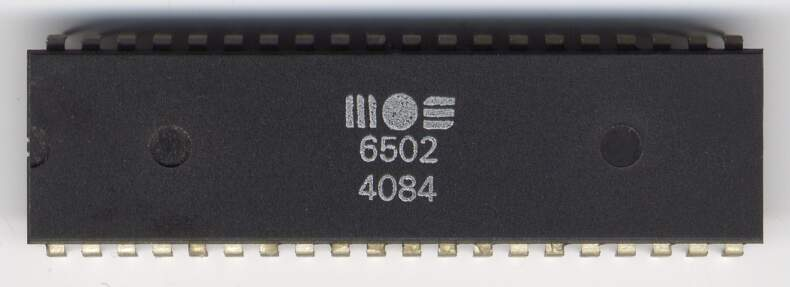
\includegraphics[width=0.7\textwidth]{6502processor.jpeg}
  \caption{Der MOS 6502-Prozessor \\ (Quelle: cpu-collection.de,
    {\small \protect\url{http://www.cpu-collection.de/?l0=i&i=198})}}
\end{figure}

Der 6502 Prozessor und seine Varianten der 6500 Familie wurde in Jahr
1975 von der Firma MOS Technology entwickelt. Er kam in legendären
Computern wie dem Apple II, dem Commodore PET und C64 zum Einsatz. Bis
heute werden Varianten davon produziert und verkauft.

Entsprechend hat er eine grosse Fangemeinde und man findet online eine
grosse Anzahl von Webseiten, die sich damit befassen, seine
Eigenschaften detailliert dokumentieren und Software zu seiner
Emulation bereit stellen.

Er war in seiner ersten Version aus 3510
Transistoren\footnote{Alternativ findet man auch die Zahl 4528, wenn
  die Pull-Up-Widerstände mitgezählt
  werden. Siehe~\cite{MOS6502BestLayoutGuy}} in CMOS-Technik aufgebaut
und wurde --- mangels entsprechender Computer --- noch von Hand
gezeichnet und danach mit foto-lithografischen Mitteln verkleinert für
die Produktion.  Seine Taktrate wurde zwischen 1\unit{MHz} und
2\unit{MHz} angegeben, je nach Version.

Eines der unglaublichsten Projekte ist eine Simulation des Prozessors
auf der physikalischen Transistor ebene. Das heisst, es wurde seine
komplette Schaltung durch \emph{reverse engeneering} bestimmt und
daraus eine virtuelle Kopie davon erstellt\cite*{thevisual6502}.

\subsection{Aufbau}

Der 6502 Prozessor hat eine Register- und damit Datenbus-Breite von 8
Bit, also 1 Byte pro Speicherstelle. Die Breite des Adressbus beträgt
16 Bit, so dass ein maximaler Hauptspeicher von
$2^{16}\unit{Byte} = 64 \unit{KiByte}$ adressiert werden kann. Dieser
Hauptspeicher wird in \emph{Seiten} zu je $2^8\byte=256\byte$
aufgeteilt, wovon die erste (mit Nummer 0, daher \emph{Zeropage}
genannt) und zweite (mit Nummer 1) spezielle Funktionen haben:

\begin{itemize}
\item Die Zeropage dient als eine Art \emph{Cache}, da deren
  Speicherstellen schneller gelesen und geschrieben werden können, als
  die der übrigen Seiten (siehe~\ref{sec:address_modes}).
\item Die zweite Seite wird als \emph{Stack} verwendet für den
  Mechanismus des Aufrufs von \emph{Subroutinen} und
  \emph{Interrupts}.
\end{itemize}

\subsection{Arithmetisch-logische Einheit}
\label{sec:alu}


Die arithmetisch-logische Einheit, kurz \emph{ALU} (von
\emph{A}rithmetic and \emph{L}ogical \emph{U}nit) des Prozessors kann
die folgenden Operationen ausführen:

\begin{itemize}
\item \emph{Addition} zweier Operanden mit Übertrag
  (\emph{carry}). Dieser Übertrag kann dazu gebraucht werden, um die
  Addition von Zahlen mit mehr als einem Byte Grösse zu programmieren.
    
\item \emph{Subtraktion} zweier Operanden mit Übertrag (\emph{carry},
  eigentlich eher \emph{borrow}, siehe~\cite{kenshirriff6502overflow}).
\item Bitweise logische Operationen \emph{Und}, \emph{Oder} und
  \emph{exklusives Oder} zweier Operanden.
    
  Interessanterweise fehlt aber die bitweise \emph{Negation}.
\item \emph{Inkrement} und \emph{Dekrement}, das heisst Erhöhen
  bzw. Vermindern eines Operanden um Eins.
\end{itemize}

\subsection{Register}
\label{sec:register}


Der Prozessor besitzt ein sehr kleine Anzahl von
\emph{Registern}, die man zu seiner Programmierung verwenden kann:

\begin{itemize}
\item Der \emph{Akkumulator}, auch \acc-Register genannt.
    
  Sein Inhalt wird für den ersten Operanden der arithmetischen und
  logischen Operationen verwendet.
\item Zwei Index-Register, \xreg- und \yreg-Register.
    
  Deren Inhalt wird für Wiederholungen bei der Verarbeitung von Listen
  gebraucht.
\item Der Programmzähler, auch \pc-Register genannt (von
  \emph{p}rogram \emph{c}ounter).

  Dieses Register kann als einziges 16\bit, also 2\byte, halten,
  besteht technisch aus zwei separaten Registern, genannt \texttt{PCL}
  und \texttt{PCH} für \texttt{P}rogram \texttt{C}ounter \texttt{L}ow,
  beziehungsweise \texttt{H}igh.
  
  Es enthält die Adresse des Befehls, der im nächsten Schritt geladen
  und ausgeführt wird.  
\item Der \emph{Stackpointer}, \stp-Register genannt.
     
  Zeigt auf die nächste freie Speicherstelle des Stacks, also der
  zweiten Speicherseite.
    
  Dieser wird von \texttt{FF} nach unten gezählt, das heisst die erste
  Stack-Speicherstelle hat die absolute Adresse \texttt{01FF}.
\item Das \emph{Statusregister}, \sreg-Register.
    
  Von dessen 8 Bit werden 7 als \emph{Flag} gebraucht, um verschiedene
  Zustände des Prozessor zu signalisieren, siehe Abschnitt~\ref{sec:flags}. 
\end{itemize}

\subsection{Status-Flags}
\label{sec:flags}

Von den acht Bits des Statusregister dienen 7 als \emph{Flags} (Markierungen)
verschiedener Zustände des Prozessors oder Ergebnisse von
Instruktionen.

So können zum Beispiel die Ergebnisse von Addition und
Subtraktion sowohl vorzeichenlos als auch mit Vorzeichen behaftet
interpretiert werden, siehe Tabelle~\ref{tab:flags}.


 
\begin{xltabular}{\linewidth}{@{}ccX@{}}
  \caption{Statusflags\label{tab:flags}}\\\toprule
  Bit Nr. & Name & Funktion \\\midrule\endhead
  0 & \texttt{C} & Das \emph{Carry}-Flag signalisiert einen Übertrag
                   bei der letzten arithmetisch-logischen Operation.
                   
    
                   Um ein korrektes Resultat zu garantieren, muss
                   dieses vor jeder Addition oder Subtraktion richtig
                   gelöscht beziehungsweise gesetzt werden. \\
  1 & \texttt{Z} & Das \emph{Zero}-Flag wird gesetzt, wenn das
                   Resultat der letzten Operation Null war.
                   

                   Dieses Flag wird nicht nur durch die
                   arithmetisch-logischen Operationen verändert
                   sondern auch durch die Befehle, die Daten 
                   aus dem Speicher in ein Register holen. \\   
  2 & \texttt{I} & Ist das \emph{Interrupt Disable}-Flag gesetzt,
                   werden normale Interrupt-Requests ignoriert. \\ 
  3 & \texttt{D} & Wenn das \emph{Decimal Mode}-Flag gesetzt ist,
                   werden die Addition und  Subtraktion durch die ALU
                   in einem speziellen  dezimalen Modus
                   ausgeführt\footnote{In der aktuellen Version dieses
                   Simulators ist dieser Modus noch nicht
                   implementiert und das \emph{D}-Flag wird
                   ignoriert.}. \\ 
  4 & \texttt{B} & Das \emph{Break}-Flag wird durch den Break-Befehl
                   gesetzt, um zu signalisieren, dass der es sich um
                   einen Software-Interrupt handelt, der nicht durch
                   die Interrupt-Leitung ausgelöst wurde. \\ 
  5 & --- & Wird nicht verwendet und kann theoretisch beim
            Programmieren des Prozessors für benutzerdefinierte Zwecke
            verwendet werden. \\ 
  6 & \texttt{V} & Das \emph{Overflow}-Flag wird für die
                   Interpretation der Addition und Subtraktion als
                   vorzeichenbehaftete Operationen verwendet. 

                   Das gesetzte \texttt{V}-Flag signalisiert, dass bei
                   einer vorzeichenbehafteten Addition das Ergebnis
                   grösser als 127, bzw.~bei einer Subtraktion kleiner
                   als -128 war\footnote{Da der Zweck dieses Flags auf
                   die Interpretation der Addition und Subtraktion als
                   vorzeichenbehaftete Operationen beschränkt ist,
                   kann es im Unterricht auch ignoriert werden}. \\ 
  7 & \texttt{N} & Das \texttt{n}-Flag wird gesetzt, wenn das
                   höchstwertige Bit nach einer Addition oder
                   Subtraktion auf 1 steht. 
  \end{xltabular}

\newpage
\section{Der Simulator}
\label{sec:der-simulator}

Die graphische Benutzeroberfläche (GUI) des 6502Simulator stellt eine
Sicht auf die relevanten Teile des 6502 Prozessors und seinen
Hauptspeicher dar, siehe Abbildung~\ref{fig:gui}.

\begin{figure}
  \centering
  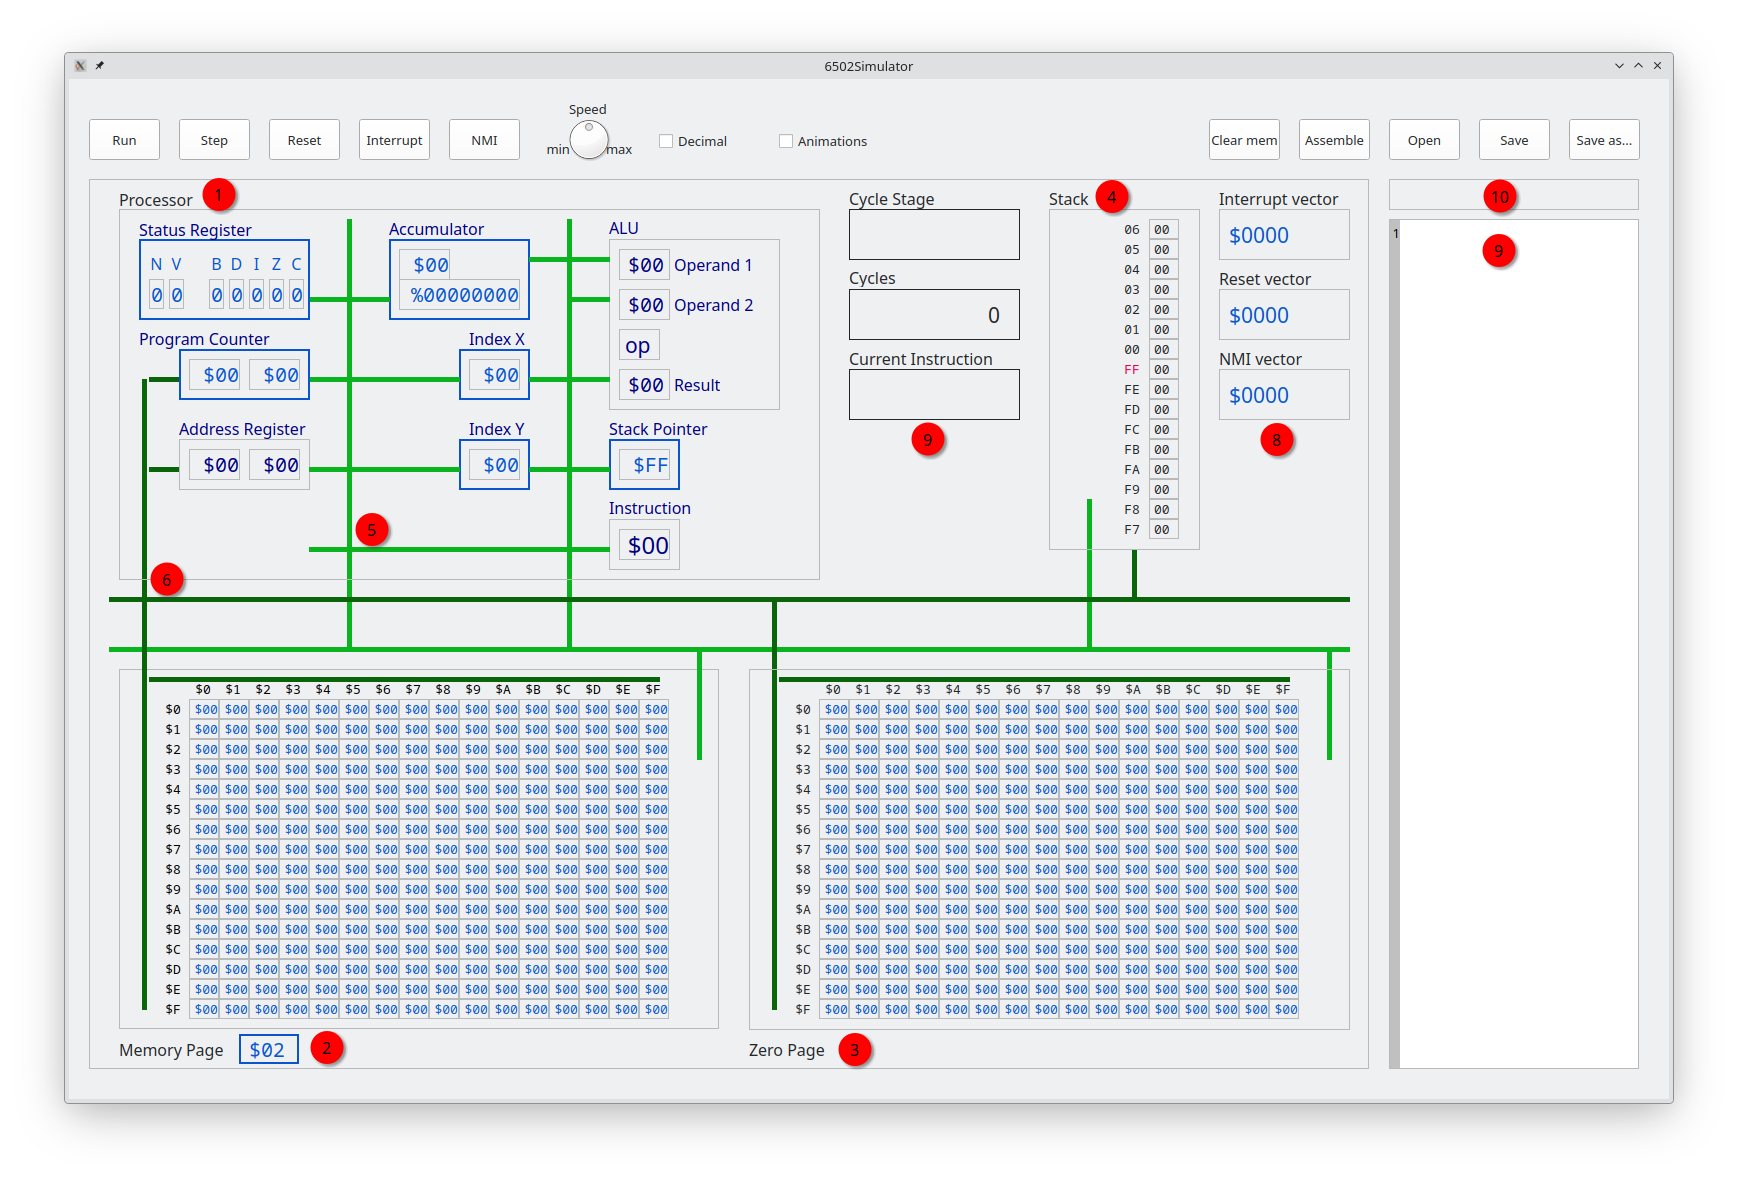
\includegraphics[width=\linewidth]{gui}
  \caption{Die GUI des 6502Simulator}
  \label{fig:gui}
\end{figure}

Es wurde versucht, die Bedienung möglichst einfach zu halten. Es gibt
kein Menü sondern nur eine kleine Reihe von Buttons oben, mit Hilfe
deren die benötigten Aktionen ausgelöst werden können. Zudem sind blau
dargestellte Elemente wie Register und Speicherstellen klickbar, um
deren Wert zu ändern. Alle numerischen Eingaben können entweder
dezimal (z. B. \lstinline!134!), hexadezimal (z. B. \lstinline!$A8!
oder \lstinline!0xFF10!)  oder binär (z. B. \lstinline!%100101! oder
\lstinline|0b11101010|) erfolgen.

\subsection{Elemente}
\label{sec:elemente}


Innerhalb des Prozessors (\picref{1} in der Abbildung~\ref{fig:gui})
sind die oben genannten Register \acc, \xreg, \yreg, \pc, \sreg\ und
\stp\ sowie die arithmetisch-logische Einheit ALU dargestellt. Der
Inhalt des Akkumulators wird zusätzlich in der binär gezeigt, um die
bitweisen logischen Operationen einfacher nachvollziehen zu können.

Zusätzlich ist das Adressregister, das die aktuell
adressierte Speicherstelle (zum Lesen oder Schreiben), und das
\emph{Instruktionsregister} gezeigt, das den zuletzt geladenen Opcode
enthält.

Der Hauptspeicher kann aus Platzgründen natürlich nicht als Ganzes
dargestellt werden:

Links unten (\picref{2} in der Abbildung~\ref{fig:gui}) sind die 256
Stellen einer Seite des Hauptspeichers matrixförmig angezeigt,
darunter ist die Nummer der angezeigten Seite ersichtlich und
wählbar. Die dargestellte Seite wechselt dynamisch während der
Ausführung eines Programms, je nach dem, auf welche Speicherstelle
gerade zugegriffen wird.


Rechts daneben (\picref{3} in der Abbildung~\ref{fig:gui}) ist in
gleicher Form der Inhalt der Zeropage dargestellt.

Für die zweite Speicherseite, die ja den Stack enthält (\picref{4} in
der Abbildung~\ref{fig:gui}), wurde eine andere, spaltenförmige
Darstellungsform gewählt: In der Mitte steht das Stack-Element, auf
das der Stackpointer aktuell zeigt (rot hervorgehoben), nach unten
nehmen die Adressen zu, nach oben ab. Die Darstellung muss man sich
kreisförmig vorstellen, da oberhalb der höchsten Adresse \hex{01FF}
wieder die tiefste Adresse \hex{0100} anschliesst.\footnote{Dies in
  Übereinstimmung der Stack-Logik, die bei einem Unterschreiten der
  \hex{00} ebenfalls wieder nach \hex{FF} springt.}

In hellgrüner Farbe wird der 8\bit\ breite Datenbus dargestellt
(\picref{5} in der Abbildung~\ref{fig:gui}, während für den 16\bit\
breiten Adressbus eine dunkelgrüne Farbe verwendet wird (\picref{6} in
der Abbildung~\ref{fig:gui}).\footnote{Es wird auf eine unterschiedliche
  Darstellung des Bus innerhalb und ausserhalb des Prozessors
  verzichtet, obwohl dies in der Realität natürlich nicht dasselbe
  ist.}

Zwischen dem Prozessor und dem Stack (\picref{7} in der
Abbildung~\ref{fig:gui} werden Informationen zum Programmablauf
angezeigt: Der momentane Schritt innerhalb des Von Neumann-Zyklus
"`fetch"', "`decode"' beziehungsweise "`run"', die Anzahl
abgearbeiteter Prozessorzyklen seit dem letzten Zurücksetzen sowie die
aktuelle Instruktion in desassemblierter Form.

Die drei Vektoren, welche die Adressen enthalten, an denen nach einem
Interrupt, einem Reset beziehungsweise einem nicht maskierbaren
Interrupt (\emph{NMI}) die Programmausführung fortgesetzt wird, sind
rechts des Stacks gezeigt und können dort verändert werden (\picref{8}
in der Abbildung~\ref{fig:gui}).

Die Elemente des Assemblers (siehe Abschnitt~\ref{sec:assembler}
zuletzt nehmen den rechten Rand des Fensters ein: ein Texteingabefeld
für den Assemblercode (\picref{9} in der Abbildung~\ref{fig:gui}) und
darüber der Name der aktuellen Assembler-Datei (\picref{10} in der
Abbildung~\ref{fig:gui}).

\subsection{Bedienung}
\label{sec:bedienung}

Die Bedienung des Simulators ist -- wie gesagt -- möglichst schlicht
gehalten.

Es gibt im Wesentlichen drei Bereiche für die Bedienung des
Simulators: 

\begin{itemize}
\item Setzen von Werten für Register und Speicherstellen, siehe oben.
\item Steuern und Darstellen des Programmablaufs.
  \begin{description}
  \item[Run]-Button: Durch Klicken darauf, wird der Programmablauf ab
    der aktuellen Adresse im Programmzähler gestartet. Das heisst die
    Instruktionen werden fortlaufend abgearbeitet.
  \item[Step]-Button: Die einzelne Instruktion an der Adresse im
    Programmzähler wird ausgeführt.
  \item[Reset]-Button: Der Prozessor wird zurückgesetzt, das heisst
    die Register \acc, \xreg, \yreg und \sreg\ werden auf \hex{00}
    gesetzt, der Stackpointer \stp\ auf \hex{FF} und der
    Programmzähler \pc\ auf den Wert des Reset-Vektors.
  \item[Interrupt]-Button: Ein externer Interrupt wird simuliert und
    die laufende Programm-Ausführung angehalten.
  \item[Speed]-Regler: Die Geschwindigkeit der Simulation kann
    gesteuert werden.
  \item[Decimal]-Checkbox: Der Inhalt von Datenregistern und
    Speicherstellen wird dezimal und nicht hexadezimal
    dargestellt.
    Der Programmzähler und das Adressregister hingegen werden immer
    hexadezimal dargestellt, genauso wie die Daten, auf dem Adressbus.
  \item[Animations]-Checkbox: Datentransfers innerhalb des Prozessors
    und zwischen dem Hauptspeicher und dem Prozessor werden durch
    Animationen visualisiert.
  \end{description}
\item Arbeiten mit Assembler-Code.
  Im grossen Text-Eingabefeld kann zeilenweise Assemblercode
  geschrieben werden, wie im Abschnitt~\ref{sec:assembler}
  beschrieben.
  
  Während der Programmausführung wird die aktuell ausgeführte Zeile
  farblich hervorgehoben.

  Damit der Code assembliert werden kann, muss er in einer Datei mit
  Endung \lstinline!.asm! gespeichert werden. Der Name der aktuellen
  Datei wird im Text-Feld darüber angezeigt.
  \begin{description}
  \item[Assemble]-Button: Die aktuelle Assembler-Datei wird
    assembliert.
    Falls die Assemblierung fehlerfrei verläuft, wird der erhaltene
    Programm-Code in den Hauptspeicher geladen.
    Andernfalls werden Fehlermeldungen angezeigt, die die Zeilen mit
    Fehlern nennen.
  \item[Open]-Button: Eine bestehende Assembler-Datei kann gewählt und
    geöffnet werden.
  \item[Save]-Button: Der in Arbeit befindliche Assembler-Code wird in
    der aktuellen Datei gespeichert.
  \item[Save as]-Button: Der in Arbeit befindliche Assembler-Code kann
    in einer neuen Datei gespeichert werden.
  \item[Clear mem]-Button: Der Hauptspeicher wird gelöscht, das heisst
    es werden alle Speicherstellen auf \hex{00} gesetzt.
  \end{description}
\end{itemize}

\newpage

\section{Instruktionen}
\label{sec:instruktionen}


Die \emph{Instruktionen} oder \emph{Befehle} des 6502 Prozessor
bestehen aus einem Byte, das \emph{Operation code} (kurz
\emph{Opcode}) genannt wird, gefolgt von bis zu zwei zusätzlichen
Bytes, die einen \emph{Operanden} angegeben.

Damit wir Menschen diese Instruktionen einfacher lesen und vor allem auch
schreiben können, werden sowohl für die Opcodes als auch für
allfällige Operanden nicht die Bytes als Zahlenwerte notiert, sondern
es werden mnemonische Schreibweisen verwendet.
Die Übersetzung dieser \emph{Mnemonics} in die Maschinensprache, also
in die entsprechenden Byte-Sequenzen nennt man \emph{Assemblierung},
die Übersetzung in der umgekehrten Richtung \emph{Desassemblierung}.


In Tabelle~\ref{tab:instruction_examples} sind eine Reihe von
Instruktionen zusammen mit ihrer mnemonischen Schreibweise aufgelistet
und kurz beschrieben. Details finden sich in den
Abschnitten~\ref{sec:instruction_set}
und~\ref{sec:address_modes}\footnote{Es macht im Unterricht sicher
  Sinn, wenn man den Einstieg mit Hilfe dieser und ähnlicher Beispiele
  macht, mit dem Simulator diese zunächst Byte für Byte in den
  Hauptspeicher schreibt, ausführen und damit visualisieren lässt.}.

\begin{longtable}{@{}llp{10cm}@{}}
  \caption{Beispiele von Instruktionen}
  \label{tab:instruction_examples} \\
    \toprule
    Instruktion &  Mnemonic & Beschreibung \endhead
    \midrule
    \lstinline!$A9 $10! & \lstinline!LDA #$1!   & Der Wert \hex{10}
                                                  wird in den
                                                  Akkumulator geladen\\           
    \lstinline!$8E $00 $20! & \lstinline!STX $0200! & Der Wert des
                                                      Index-Registers
                                                      \xreg\ wird an die
                                                      Speicherstelle
                                                      \hex{200}
                                                      geschrieben. \\
    \lstinline!$65 $B0! & \lstinline!ADC $B0! & Der Wert in der
                                                Speicherstelle
                                                \hex{00B0} wird zum
                                                Akkumulator \acc\ addiert
                                                unter Berücksichtigung
                                                des Carry-Flags C \\
    \lstinline!$88! & \lstinline!DEY! & Der Wert des Index-Registers \yreg\
                                        wird um 1 verkleinert
                                        (decrement) \\
    \lstinline!$6C $34 $12! & \lstinline!JMP ($1234)! & Die
                                                       Programmausführung
                                                       wird ab der
                                                       Stelle
                                                       fortgesetzt,
                                                       deren Adresse an
                                                       den Speicherstellen
                                                       \hex{1234} und
                                                       \hex{1235}
                                                        steht. \\
    \lstinline!$10 $08! & \lstinline!BPL *10! & Fall der \nflag-Flag nicht
                                                gesetzt ist, werden die nächsten
                                                8 Byte in der
                                                Programmausführung
                                                übersprungen.

                                                In der mnemonischen
                                                Schreibweise steht
                                                dafür \texttt{*10}, weil 2
                                                Bytes schon durch die
                                                Anweisung selbst
                                                benötigt werden.\\
    \lstinline!$AA! & \lstinline!TAX! & Kopiere den Wert des
                                        Akkumulators \acc\ in das
                                        Index-Register \xreg. \\
    \bottomrule
  \end{longtable}


\subsection{Adressierungsarten}
\label{sec:address_modes}

Viele Instruktionen brauchen einen zusätzlichen Operanden. Dieser wird
in einem bis zwei zusätzlichen Adressbytes angegeben, die nach dem Opcode
folgen. Der Opcode zusammen mit den Adressbytes machen zusammen die
Instruktion aus.   

Der 6502 Prozessor kennt eine Reihe von verschiedenen
\emph{Adressierungsarten} (\emph{Address mode}), die beschreiben, wie
aus den Adressbytes letztlich der Operand bestimmt wird.
Tabelle~\ref{tab:address-modes} gibt einen Überblick all dieser
Adressierungsarten\footnote{Im Unterricht wird es nicht möglich
  sein, alle diese Adressierungsarten anzuschauen.  Sie sind in daher
  in absteigender Wichtigkeit (für den Unterricht) in der Tabelle
  aufgelistet.

  Die indirekten Adressierungsarten können zum Beispiel ohne grossen
  Schaden weggelassen werden.

  Da der Assembler (siehe Abschnitt~\ref{sec:assembler}) uns die
  Berechnungen der relativen Adressierung bei Verzweigungsbefehlen
  abnimmt, kann auch darauf verzichtet werden, deren Details
  anzuschauen.}.
  

\begin{xltabular}{\linewidth}{@{}p{25mm}Xl@{}}
  \caption{Adressierungsarten \label{tab:address-modes}}\\\toprule
  \textbf{\sffamily Bezeichnung} \lstinline!Mnenomic! & Beschreibung & Grösse\\\midrule\endhead 
  \textbf{\sffamily Implicit}\newline \impl &
             Implizite Adressierung
             
             Dabei sind die Operanden implizit im Befehl beinhaltet und es werden
             keine weitere Operanden benötigt.
                      &  1\byte \\
   \multicolumn{3}{p{11.5cm}}{
     \begin{tabularx}{1.2\linewidth}{lX}\midrule
       \lstinline!TXS! & Kopiere das \xreg-Register in das \sreg-Register\\
       \lstinline|CLC| & Lösche das \cflag-Flag, \\
       \lstinline|INC| & Erhöhe den Wert des Akkumulators\\
     \end{tabularx}}  
  \\\midrule
  \textbf{\sffamily Immediate}\newline \imm & Unmittelbare Adressierung
  
  Ein nachfolgendes Byte direkt als nummerischer Wert
  interpretiert.
  
  Es handelt sich also nicht um eine Adresse im
  eigentlichen Sinn.
  & 2\byte \\
  \multicolumn{3}{p{11.8cm}}{
  \begin{tabularx}{1.2\linewidth}{lX}\midrule
    \lstinline!LDX \#$10! & Lade den Wert \hex{10} in das \xreg-Register \\
    \lstinline!ADC \#$80! & Addiere den Wert \hex{80} zum Akkumulator \acc \\
    \lstinline!AND \#$01! & Bitweises Und des Akkumulators mit dem Wert \hex{1} \\
    \lstinline|CPY \#$80| & Vergleiche das \yreg-Register mit dem Wert \hex{80} \\
  \end{tabularx}} \\\midrule
  \textbf{\sffamily Absolute}\newline \abs\newline\textbf{\sffamily Zeropage}\newline \zp
       & Absolute Adressierung
             
         Hier wird geben zwei Byte nach dem Opcode die vollständige Speicher-Adresse an,
         an der der Operand steht.

         Wird nur ein Byte angegeben, wird dieses als Adresse
         innerhalb der ersten Speicherseite interpretiert und man spricht man von
         Zeropage-Adressierung.
                      & 3\byte/2\byte \\
  \multicolumn{3}{p{11.8cm}}{
  \begin{tabularx}{1.2\linewidth}{lX}\midrule
    \lstinline!LDX \$4010! & Lade den Wert an der Adresse \hex{4010} in das \xreg-Register \\
    \lstinline!STY \$FF! & Speichere den Wert des \yreg-Registers in der Adresse \hex{00FF} \\
  \end{tabularx}} \\\midrule
  \textbf{\sffamily Absolute\newline indexed} \absx, \absy\newline
  \textbf{\sffamily Zeropage\newline indexed}\newline \zpx, \zpy &
                                Absolute Adressierung mit
                                \xreg-Indexierung beziehungsweise
                                \yreg-Indexierung. 
                     
                                Hierbei wird zu der Adresse, die in
                                den beiden folgenden Bytes steht, noch
                                der Wert des \texttt{X}, bzw.\
                                \texttt{Y}-Registers als Index addiert.

                                Wie bei \abs gibt es davon auch die
                                entsprechenden Zeropage-Varianten, bei
                                denen wiederum nur ein Byte verwendet
                                wird, um eine Adresse innerhalb der
                                ersten Speicherseite anzugeben.
                      & 3\byte/2\byte \\
  \multicolumn{3}{p{11.8cm}}{
  \begin{tabularx}{1.2\linewidth}{lX}\midrule
    \lstinline!STA \$2000,X! & Ist der Wert des Index-Registers \xreg\ gleich \hex{A0},
                               so wird der Wert des Akkumulators an der Stelle \hex{20A0}
                               gespeichert. \\
    \lstinline!LDA \$F0,X! & Ist der Wert des Index-Registers \xreg\ gleich \hex{0044},
                             so wird an der Stelle \hex{34} in den Akkumulator \acc
                             geladen. Beachte, dass eigentlich
                             $\hex{F0}+\hex{44} =\hex{134}$ ist.
                             Der Übertrag wird also ignoriert!
    \end{tabularx}} \\\midrule

  \textbf{\sffamily Indirect}\newline \ind & Indirekte Adressierung
             
             Es wird mit zwei Bytes eine Speicherstelle angegeben, an der die
             effektive Adresse des Operanden beginnt (das heisst, das \lobyte
             steht an dieser Adresse, das \hibyte\ in der darauf
             folgenden). & 3\byte \\ 
  \multicolumn{3}{p{11.8cm}}{
  \begin{tabularx}{1.2\linewidth}{lX}\midrule
    \lstinline!JMP (\$1234)! & Steht an der Stelle \hex{1234} der Wert \hex{10}
                               und an der darauf folgenden Stelle \hex{1235} der Wert \hex{A8},
                               so wird an die Stelle \hex{A810} gesprungen (der Wert \hex{A810} in
                               den Programmzähler geladen).
    \\
    \end{tabularx}} \\\midrule
  \textbf{\sffamily X-Indexed\newline Indirect}\newline \indx &
                           Indirekte Adressierung mit \xreg-Indexierung
                           
                           Bei dieser Adressierungsart wird -- wie bei
                           \zpx\ -- zuerst das nachfolgende Byte zum
                           \xreg-Register addiert. Danach wird der erhaltene
                           Wert verwendet, um den Start der vollständigen
                           Adresse (zwei Byte in \emph{little endian}-Ordnung)
                           des Operanden zu erhalten.  & 2\byte \\
  \multicolumn{3}{p{11.8cm}}{
    \begin{tabularx}{1.2\linewidth}{lX}\midrule
      \lstinline!STA (\$A0,X)! & Steht an der Stelle \hex{A0} der Wert \hex{40} und hat
                                 Indexregister \xreg\ den Wert \hex{0A}, so werden die
                                 Werte an den Stellen \hex{4A} und \hex{4B} verwendet.
                                 Sind diese \hex{00} und \hex{20}, so wird der Wert des
                                 Akkumulators an die Stelle \hex{2000} des Speichers
                                 geschrieben.
    \\
    \end{tabularx}} \\\midrule
  \textbf{\sffamily Indirect\newline Y-Indexed}\newline \indy &
                           \yreg-Indexierte indirekte Adressierung

                           Bei dieser indirekten Adressierungsart, wird zuerst
                           das nachfolgende Byte verwendet, um eine vollständige
                           Adresse (2 Byte in \emph{little endian} Ordnung)
                           innerhalb der Zeropage zu bestimmen.
                           Anschliessend wird zu dieser Adresse noch der Wert
                           des Indexregister \yreg\ addiert, um die definitive
                           Adresse des Operanden zu erhalten. & 2\byte \\
  \multicolumn{3}{p{11.8cm}}{
     \begin{tabularx}{1.2\linewidth}{lX}\midrule
      \lstinline!LDA (\$70),Y! & Steht an der Stelle \hex{70} der Wert \hex{B1} und
                                 danach an der Stelle \hex{71} der Wert \hex{35} und hat
                                 Indexregister \xreg\ den Wert \hex{20}, so ist der
                                 adressierte Operand \hex{35B1}+\hex{20}=\hex{35D1}.
    \\
    \end{tabularx}}  \\\midrule
  \textbf{Akkumulator}\newline \acc & Adressierung des Akkumulators

                         Einige wenige Instruktionen adressieren den
                         Akkumulator separat. Diese Adressierungsart
                         entspricht im wesentlichen der impliziten. &
                                                                      1\byte\\
  \multicolumn{3}{p{11.8cm}}{
    \begin{tabularx}{1.2\linewidth}{lX}\midrule
       \lstinline!ASL A! & Schiebt die Bits des Akkumulators um eine
                          Stelle nach links    \\
    \end{tabularx}} \\\bottomrule
\end{xltabular}

\subsection{Befehlssatz}
\label{sec:instruction_set}

Der Befehls- oder Instruktionssatz des 6502 Prozessor ist relativ
klein. Es gibt insgesamt 56 verschiedene Instruktionen, die zum Teil
mehrere Adressierungsarten für ihre Parameter kennen. Daraus ergibt
sich ein Total von 151 verwendeten \emph{Opcodes} von den 256
möglichen.

Die restlichen Opcodes sind sogenannt \emph{illegal} und nicht
offiziell dokumentiert. Einige davon kann man tatsächlich für eher
exotische Zwecke nutzbar machen (siehe??). Der vorliegende Emulator
behandelt sie aber alle als \emph{No operation} \texttt{NOP}, also als
Befehle ohne Effekt.\footnote{Dies aus didaktischen Gründen, um den
  Einstieg in die Assemblerprogrammierung nicht unnötig zu
  verkomplizieren.}.

Einen Überblick über den vollständigen Befehlssatz zusammen mit den jeweiligen Adressierungsarten findet sich in den Tabellen des Anhangs~\ref{sec:instruction_reference}.

\subsubsection{Datentransfer}
\label{sec:datatransfer_instructions}
Zu den wichtigsten Aufgaben eines Programms gehört das Kopieren von
Daten von einer Speicherstelle zu einer anderen. Der 6502 kennt dafür
eine Reihe von Befehlen.

\begin{itemize}
\item \texttt{LDA}, \texttt{LDX}, \texttt{LDY} dienen zum Laden eines
  Bytes in die Register \texttt{A}, \texttt{X}, \texttt{Y} respektive.

  Diese Operationen beeinflussen zudem alle die Flags \zflag\ und \nflag,
  je nach dem, ob die transferierten Werte Null
  bzw. negativ~\footnote{Auf vorzeichenbehaftete Arithmetik wird in
    dieser Dokumentation nicht näher eingegangen.
    
    Es genügt anzugeben, dass dabei die Zahlen in 2er-Komplement
    Darstellung interpretiert werden und dass somit Bytes, deren erstes,
    also höchstwertiges Bit 1 ist, als negativ angesehen werden.
    
    Beim Unterricht z. B. in P/AM-Klassen kann dies natürlich zum Anlass
    genommen werden, diese 2er-Komplement Darstellung zu repetieren.}
  sind.
\item \texttt{STA}, \texttt{STX}, \texttt{STY} dienen zum Speichern
  des Bytes in einem der  Register \texttt{A}, \texttt{X}, respektive
  \texttt{Y} an einer Speicherstelle des RAM.
\item \texttt{TAX}, \texttt{TAY}, \texttt{TXA}, \texttt{TYA}
  \texttt{TSX}, \texttt{TSX}, kopieren das Byte des erstgenannten
  Registers in das zweitgenannte Register.

  Diese Befehle setzen je nach Wert wieder die Flags \zflag\ und \nflag. 
\end{itemize}



Eine Übersicht über diese Instruktionen mit ihren Adressierungsarten
und zugehörigen Opcodes, findet man in
Tabelle~\ref{tab:datatransfer_instructions}.


\subsubsection{Arithmetisch-logische Operationen}
\label{sec:arithmetic_logic}

Der 6502 kennt eine Reihe von Instruktionen, die arithmetische
Operationen (Addition und Subtraktion\footnote{Multiplikation und
  Division sind nicht implementiert.

  Diese sind aufwändig in der Hardware-Implementierung und blieben
  lange Zeit spezialisierten externen Coprozessoren überlassen
  (Referenz?).

  Entgegen der intuitiven Annahme gehören die arithmetischen
  Operationen auch nicht zu den am häufigst verwendeten in der
  Programmierung.}, schrittweise Vergrösserung und
Verkleinerung\footnote{Dieses Inkrementieren und Dekrementieren eines
  Werts sind in der Programmierung so häufig verwendete Operationen,
  dass sich die Definition dedizierter Befehle dafür lohnt.

  Ausserdem entfällt dabei die Angabe eines Operanden, der immer 1
  ist.}),
und bitweise logische Operationen durchführen. Details
entnimmt man der Tabelle~\ref{tab:arithmetic_logic}.

\begin{itemize}
\item \lstinline|ADC| (\texttt{AD}dition with \texttt{C}arry) führt
  eine Addition mit Übertrag durch und \lstinline!SBC!
  (\texttt{S}u\texttt{B}traction with \texttt{C}arry) eine Subtraktion
  mit Übertrag.
  
  Damit diese die erwarteten Ergebnisse liefern, muss vor der Addition das
  Carry-Flag \cflag\ gelöscht und vor der Subtraktion gesetzt
  werden. 
  
  Der Übertrag dient dazu, die arithmetischen Operationen auch mit
  mehr als einem Byte durchführen zu können.
\item Für das schrittweise Erhöhen und Vermindern eines Registers um
  1\footnote{Im Gegensatz zu der allgemeinen Addition und Subtraktion
    sind dies in der Programmierung sehr häufig verwendete
    Operationen und werden insbesondere bei Wiederholungen und bei der
    Bearbeitung von Listen überall gebraucht.} gibt es die
  spezialisierten Befehle \lstinline|INC| (für \texttt{INC}rement),
  \lstinline|INX| (\texttt{IN}crement \texttt{X}-register) und
  \lstinline|INY| (\texttt{IN}crement \texttt{Y}-register) respektive
  \lstinline|DEC| (\texttt{DEC}rement),
  \lstinline|DEX| (\texttt{DE}crement \texttt{X}-register) und
  \lstinline|DEY| (\texttt{DE}crement \texttt{Y}-register)\footnote{Diese
    Inkrement- und Dekrement-Operationen sind zyklisch in dem Sinne,
    dass ein Inkrement des grössten Wert \hex{FF} wieder \hex{00}
    ergibt und umgekehrt ein Dekrement des kleinsten Werts \hex{00}
    das Resultat \hex{FF} liefert.}
\item Die bitweisen logische Operationen Und, Oder und exklusives Oder
  sind mit den Instruktionen \lstinline|AND|, \lstinline|ORA| (von
  \texttt{OR} with \texttt{A}ccumulator) 
  beziehungsweise \lstinline|EOR| (von \texttt{E}xclusive \texttt{OR})
  möglich\footnote{Wie erwähnt fehlt
    die bitweise Negation oder Inversion.

    Es ist eine sinnvolle Übung, zu überprüfen, dass diese durch ein
    bitweisen exklusives Oder mit dem Operanden \hex{ff} ersetzt
    werden kann.}. Diese operieren alle mit dem Akkumulator \acc\ und
  einem weiteren Wert, der durch den Operanden gegeben ist.
\item Für bitweises Schieben nach links gibt es den Befehl
  \lstinline|ASL| (\texttt{A}rithmetic \texttt{S}hift \texttt{L}eft)
  und nach rechts den Befehl \lstinline|LSR| (\texttt{L}ogical
  \texttt{S}hift \texttt{R}ight); 
  sollen die Bits aber rotiert werden, verwendet man die Befehle
  \lstinline|ROL| (\texttt{RO}tate \texttt{L}eft) beziehungsweise
  \lstinline|ROR| (\texttt{RO}tate \texttt{R}ight).
\end{itemize}


\subsubsection{Sprungbefehle}
\label{sec:branch_instructions}

Die Aufgabe dieser Kategorie von Instruktionen ist die Manipulation
des Programmzählers, und den Programmablauf zu kontrollieren.
Auf diese Weise können bedingte Anweisungen,
Programmschleifen und Unterprogramme umgesetzt werden.

\begin{itemize}
\item Der \lstinline|JMP|-Befehl (von \texttt{J}u\texttt{MP}) lädt
  einen Wert der Länge 2\byte\ in den Programmzähler und bewirkt so
  eine einfache Verzweigung des Programmablaufs.
\item Der \lstinline|JSR|-Befehl (von \texttt{J}ump to
  \texttt{S}ub\texttt{R}outine) tut dasselbe, der Programmzähler wird aber
  zusätzlich auf den Stack geschoben\footnote{Effektiv werde die 2 Byte des
    Programmzähler in der Reihenfolge \hibyte-\lobyte auf den
    Stack geschoben}, damit der Rücksprung an die
  Stelle nach dieser Anweisung möglich ist.
\item Mit dem \lstinline|RTS|-Befehl (von \texttt{R}e\texttt{T}urn from
  \texttt{S}ubroutine) kann aus einem Unterprogramm die
  Programmausführung nach der Stelle des Aufrufs fortgesetzt werden.
\item Die bedingten Verzweigungsbefehle \lstinline|BEQ| (für
  \texttt{B}ranch on \texttt{EQ}ual), \lstinline|BNE| (für \texttt{B}ranch
  on \texttt{N}ot \texttt{E}qual), \lstinline|BMI| (für \texttt{B}ranch on
  \texttt{MI}inus), \lstinline|BPL| (für \texttt{B}ranch on
  \texttt{PL}us)\footnote{Eigentlich müsste es "`branch on not minus"'
    heissen!}, \lstinline|BCS| (für \texttt{B}ranch on \texttt{C}arry
  \texttt{S}et), \lstinline|BCC| (für \texttt{B}ranch on \texttt{C}arry
  \texttt{C}lear) und zuletzt \lstinline!BVS! beziehungsweise
  \lstinline!BVC! lassen die Programmausführung an eine neue Stelle im
  Hauptspeicher verzweigen, je nach dem, ob das Flag \zflag, \nflag\,
  \cflag\ respektive \vflag\ gesetzt (1) oder gelöscht (0) ist.

  Die Distanz zum Ziel der Verzweigung muss dabei zwischen -128 und
  +127 liegen\footnote{Diese Verzweigungsbefehle verwenden als einzige
    eine relative Adressierungsart. Die Beschränkung kommt daher, dass
    dabei die Sprungdistanz als vorzeichenbehafteter Integer interpretiert
    wird.

    Da der Assembler aber deren Berechnung übernimmt, können die
    Details hier getrost weggelassen werden.}.
\end{itemize}


\subsubsection{Flag-Manipulation}
\label{sec:flag-manipulation}

Der 6502 Prozessor verfügt zudem über eine Reihe von Befehlen, deren
Hauptzweck es ist die Status-Flags zu setzen oder löschen.

\begin{itemize}
\item Die Befehle \lstinline|CLC| (von \texttt{CL}ear \texttt{C}arry
  flag), \lstinline|SEC| (von \texttt{SE}t \texttt{C}arry flag),
  \lstinline|CLD| (von \texttt{CL}ear \texttt{D}ecimal flag),
  \lstinline!SED! (von \texttt{SE}t \texttt{D}ecimal flag) und
  \lstinline|CLV| (von \texttt{CL}ear o\texttt{V}erflow) löschen
  beziehungsweise setzen das entsprechende Flag direkt.
\item Mit Hilfe der drei Vergleichsbefehle \lstinline|CMP| (für
  \texttt{C}o\texttt{MP}are), \lstinline|CPX| (für
  \texttt{C}om\texttt{P}are \texttt{X}-register) und \lstinline|CPY|
  (für \texttt{C}om\texttt{P}are \texttt{Y}-register) kann der Inhalt
  eines der drei Register mit einem anderen Wert verglichen werden.

  Sind die Werte gleich, wird sowohl das Null-Flag \zflag\ als auch
  das Carry-Flag \cflag\ gesetzt, ist der Wert im Register grösser,
  wird das \cflag-Flag gesetzt und das \zflag-Flag gelöscht. Ist der
  Wert im Register kleiner, wird sowohl das \cflag-Flag als auch
  \zflag-Flag gelöscht\footnote{Der gleiche Effekt auf das
    Statusregister kann auch durch die Subtraktion erreicht werden.
    
    Intern sind diese Vergleichs-Operationen in der ALU effektiv via
    Subtraktion implementiert. Sie haben aber den Vorteil, dass man
    durch sie den Wert im Register nicht verliert.}.
\end{itemize}

\subsubsection{Stack-Operationen}
\label{sec:stack-operationen}

Der 6502 Prozessor verfügt über einen Stapel-Bereich (\emph{stack}),
der in der zweiten Speicherseite angelegt ist, also die Adressen
\hex{01FF} hinunter bis \hex{0100} belegt.

Dabei enthält das Stack-Register \stp\ immer das \lobyte{} der Adresse
des nächsten freien Speicherplatz\footnote{Man sagt, das
  Stack-Register \emph{zeige} auf diese Adresse, weshalb dieses etwa
  auch \emph{stack pointer} genannt wird} innerhalb dieses Bereichs
und wird jedes Mal dekrementiert, wenn ein Element auf dem Stack
abgelegt wird (\emph{push}) verkleinert und umgekehrt jedes Mal
inkrementiert, wenn ein Element vom Stack geholt wird
(\emph{pop})\footnote{Die Datenstruktur des \emph{stack}, die nach dem
  \emph{LIFO}-Prinzip (\emph{l}ast \emph{i}n, \emph{f}irst \emph{o}ut
  funktioniert und die beiden elementaren Operationen \emph{push} und
  \emph{pop} kann an dieser Stelle thematisiert oder vertieft werden,
  sofern es die zur Verfügung stehende Zeit erlaubt} .

\begin{itemize}
\item Die Instruktionen \lstinline|PHA| und \lstinline|PHP| schieben
  den Akkumulator \acc\ beziehungsweise den Programmzähler \pc\ auf
  den Stack\footnote{Die beiden Bytes des Programmzählers werden in
    ??-Manier, also zuerst das \lobyte und danach das \hibyte, auf den
    Stapel geschoben.}.
\item Umgekehrt holen die Instruktionen \lstinline|PLA| und
  \lstinline|PLP| den Wert des Akkumulators beziehungsweise
  Programmzählers wieder vom Stack.
\end{itemize}

\subsubsection{Interrupts}
\label{sec:interrupts}

Unterbrechungen des Programmablaufs werden durch so genannte
Interrupts ermöglicht, wobei zwischen Hardware- und
Software-Interrupts unterschieden wird\footnote{Das ganze Thema der
  Interrupt-Behandlung geht sicher über das hinaus, was sinnvollerweise
  im obligatorischen Fach Informatik behandelt werden kann, und wird
  hier nicht ausführlich beschrieben. Für eine umfassende Darstellung
  sei zum Beispiel auf~\cite{6502org_interrupts} verwiesen}.

Der Befehlssatz des 6502 Prozessor kennt zwei Instruktionen für den
Umgang damit:

\begin{itemize}
\item \lstinline|BRK| (für \texttt{BR}ea\texttt{K} löst einen
  Software-Interrupt aus. Dabei werden der (um 2 vergrösserte)
  Programmzähler und anschliessend das Statusregister \sreg\ auf den
  Stapel geschoben und anschliessend der NMI-Vektor in den
  Programmzähler geladen.

\item \lstinline|RTI| (für \texttt{r}e\texttt{t}urn from
  \texttt{i}nterrupt) ermöglicht den Rücksprung nach der Beendigung
  eines Programmteils für die Interrupt-Behandlung. Hier werden in
  umgekehrter Reihenfolge zuerst das Statusregister \sreg\ und danach
  der Programmzähler vom Stapel geholt, was bewirkt, dass die
  Programmausführung am Ort fortgesetzt wird, wo der Interrupt  stattgefunden hatte.
\end{itemize}

\subsubsection{Vermischte Instruktionen}
\label{sec:misc_instructions}

Zuletzt seien noch die Befehle erwähnt, die nicht natürlich in eine
der obigen Kategorien fallen:

\begin{itemize}
\item \lstinline!NOP! (von \texttt{N}o  \texttt{OP}eration) tut genau
  das, was der Name sagt, nämlich nichts.
\item Der Befehl \lstinline!BIT! (für \texttt{BI}t \texttt{T}est)
  testet einige Bits seines Operanden\footnote{Die genauen
    Spezifikationen dieser einigermassen exotischen Instruktion werden
    hier übergangen und können zum Beispiel bei~\cite{6502org_instructions}
    nachgeschlagen werden.}.
\end{itemize}


\newpage
\section{Der Assembler}
\label{sec:assembler}

Der Simulator verfügt über einen einfachen Assembler, der das
Erstellen von Programmen vereinfacht. Bei dessen Implementierung habe
ich mich bei dem Quellcode von James Salvino als Vorlage bedient
(siehe~\cite{6502Asm}), diesen aber weitgehend umstrukturiert und neu
implementiert. Dies zuerst, um ihn überhaupt zu verstehen, und danach
um einige Bugs zu eliminieren, verständlichere Fehlermeldungen zu
haben und ihn an meine Bedürfnisse für den vorliegenden Simulator
anzupassen.


\subsection{Instruktionen}
\label{sec:ass_instructions}


Der Hauptzweck des Assemblers besteht zunächst darin, Instruktionen
mit den üblichen, oben beschriebenen mnemonischen Schreibweisen in der
Reihenfolge ihrer Ausführung hinschreiben zu können.

\begin{center}
  \lstinputlisting[caption={Assembler,
    Instruktionen},label=ex_insructions]{instructions.asm}
\end{center}

Durch dieses Programm werden die drei Anweisungen \lstinline!LDA #100!
(2\byte), \lstinline!ADC $FF00! (3\byte) und \lstinline!STA $FF!
(2\byte) nach einander in die Stellen 0 bis 6 des Hauptspeichers
geschrieben.

Alles, was nach einem Semikolon folgt, wird als \emph{Kommentar}
betrachtet durch den Assembler ignoriert.

Gross- und Kleinschreibung ist dabei unwichtig, es empfiehlt sich
jedoch aus Gründen der Leserlichkeit, sich auf eine einheitliche
Schreibweise festzulegen. Ebenso werden Leerzeichen am Anfang und Ende
jeder Zeile, sowie gänzlich leere Zeilen ignoriert. Auch hier
erleichtert Einheitlichkeit das Lesen und Verstehen enorm.


Daneben kennt der Assembler eine handvoll \emph{Direktiven}, die der
Programmiererin gerade bei Sprungbefehlen und beim Umgang mit Daten
das Leben deutlich einfacher machen können.

\subsection{Die \texttt{.org}-Direktive}
\label{sec:org_directive}

Beginnt eine Zeile mit der Direktive \lstinline!.org! (für
\emph{org}anize) gefolgt von einer gültigen Memory-Adresse, so fügt
der Assembler die folgenden Zeilen ab dieser Adresse in den Speicher
ein:

\begin{center}
  \lstinputlisting[caption={Assembler,
    \lstinline!.org!-Direktive},label=ex_org_directive]{org-directive.asm}
\end{center}

Die Anweisungen, um 1 und 1 zu addieren, stehen an den Adressen 512,
513, 514 und 515 im Hauptspeicher.

Ist gewünscht, dass die Programmausführung damit beginnt, muss
zusätzlich der Reset-Vektor auf diesen Wert $\hex{200}=512$ gesetzt
werden.

\subsection{Die \lstinline!.db!-Direktive}
\label{sec:db-directive}

Die Direktive \lstinline!.db! (für \emph{d}efine \emph{b}yte)
ermöglicht es, ab der aktuellen Speicherstelle eine Reihe von Werten
als Daten zu schreiben:

\begin{center}
  \lstinputlisting[caption={Die
    \lstinline+.db+-Direktive},label=ex_db_directive]{db-directive.asm}
\end{center}

Dadurch werden die sechs Werte $16$ (der Wert der Hexadezimalzahl
$\hex{A}$), $100$, $65$ (der ASCII-Code des Buchstaben 'A'), $66$,
$67$ und $13$ (der Wert der Binärzahl $\bin{1101}$) ab der Stelle
$\hex{A000}=40960$ in den Speicher geschrieben.

\subsection{Die \lstinline!.ds!-Direktive}
\label{sec:ds_directive}

Mit Hilfe der Direktive \lstinline!.ds! kann eine Anzahl Byte als
Speicherplatz reserviert werden.

\begin{center}
  \lstinputlisting[caption={Die
    \lstinline+.ds+-Direktive},label=ex_ds_directive]{ds-directive.asm}
\end{center}

Dadurch werden in den ersten fünf Bytes des Hauptspeichers die beiden
Instruktionen 16 Byte frei gelassen. Die nächste Instruktion beginnt
daher an der Stelle $\hex{15}=21$ des Hauptspeichers.


\subsection{Die \lstinline!.equ!-Direktive}
\label{sec:equ_directive}

Die Direktive \lstinline!.equ! Namen für Speicheradressen zu
definieren.

\begin{center}
  \lstinputlisting[caption={Die
    \lstinline+.equ+-Direktive},label=ex_equ_directive]{equ-directive.asm}
\end{center}

Es werden zuerst die Werte, die nacheinander an den Speicherstellen
\hex{AA00} und \hex{AA01} stehen addiert und anschliessend der Wert an
der Speicherstelle \hex{AAB0} subtrahiert. Beachte, dass vor den
arithmetischen Operationen das \lstinline|C|-Flag richtig gesetzt
wird.




\subsection{Labels}
\label{sec:ass_labels}

Die nächste Erleichterung, die der Assembler bietet, ist die
Möglichkeit, die aktuelle Speicheradresse mit einem Namen
(\emph{Label}) zu versehen, und diese dann damit anzusprechen.
Dies ist insbesondere für den relativen Adressierungsmodus hilfreich,
da man so nicht mehr bei jeder Änderung die Sprungweite selbst neu
berechnen muss. 

Ein Label muss mit einem Buchstaben beginnen, gefolgt von bis zu 7
weiteren Buchstaben oder Ziffern\footnote{Ausgeschlossen ist zudem das
  Label, das nur aus dem Buchstaben \lstinline!A! besteht, wegen der
  Verwechslung mit dem Adressierungsart \acc}.

\begin{center}
  \lstinputlisting[caption={Labels 1},label=ex_label1]{label1.asm}
\end{center}

Das Programmfragment führt eine Schleife 10 Mal aus, indem in die
Speicherstelle der 2. Zeile mit dem Namen \lstinline!loop! versehen
und dann in der 3. Zeile dorthin verzweigt wird, bis das Indexregister
\lstinline!X! den Wert 0 enthält.

Zudem ist einfache Arithmetik mit einem Label möglich, das heisst, man
kann zu einem solchen entweder eine feste Zahl addieren oder davon
subtrahieren.


\begin{center}
\begin{lstlisting}[caption={Assembler, Beispiel 3}, label=asmbeisp3]
paar .db 10,15

LDA paar
LDX paar+1
STA paar+1
STX paar
\end{lstlisting}
\end{center}

Das Programmfragment vertauscht den Inhalt von zwei aufeinander
folgenden Speicherstellen.

\newpage
\section{Beispiele}
\label{sec:beispiele}

Im folgenden werden einige kurze Beispielprogramme gezeigt, die
wichtige Konzepte und \emph{Best Practices} der
Assembler-Programmierung zeigen sollen.

\subsection{Vorlage}
\label{sec:vorlage}

Es lohnt sich, für Übungen und Aufgaben eine Vorlage zu haben, die
ein einheitliches Erscheinungsbild der Programme erleichtern und eine
einfache Handhabung in der GUI ermöglichen:

\lstinputlisting[caption={Vorlage},label=ex_template]
{~/Python/6502Simulator/examples/template.asm}

Der Einstiegspunkt für das ausführbare Programme wird hier als
\hex{0200} gewählt, also am Beginn der Speicherseite 2. Dieser wird
zuletzt an die Stellen \hex{FFFC} und \hex{FFFD} des Speichers
geschrieben, wo der Reset-Vektor des Prozessors steht\footnote{In
  bekannter \emph{little endian} Manier.}. Auf diese Weise, startet
die Programmausführung nach einem Reset immer an der gewünschten
Stelle.



\subsection{Maximum von zwei, drei oder mehr Werten}
\label{sec:example_max}

Den grösseren von zwei Werten kann man einfach durch Vergleichen der
beiden bestimmen:
\lstinputlisting[caption={Maximum von 2 Werten}, label=ex_max_two]{~/Python/6502Simulator/examples/max_two.asm}
 
Will man den grössten von drei Werten bestimmen, bestimmt man zuerst das Maximum der ersten beiden und vergleicht dieses anschliessend mit dem dritten Wert:
\lstinputlisting[caption={Maximum von 3 Werten}, label=ex_max_two]{~/Python/6502Simulator/examples/max_three.asm}

Dies lässt sich nun auf $n$ viele Werte verallgemeinern: Das erste
Maximum ist der erste Wert in der Liste, danach vergleicht man alle
folgenden Werte mit dem bisherigen Maximum und passt dieses an, wenn
man einen Wert findet der noch grösser ist\footnote{Damit hat
  man den bekannten \emph{Bubble Sort}-Algorithmus implementiert.}:
\lstinputlisting[caption={Maximum einer Liste von Werten}, label=ex_max_two]{~/Python/6502Simulator/examples/max_lst.asm}

Man beachte das Verwenden des Index-Registers \xreg\ zusammen mit der
indexierten Adressierungsart \indx, um die Elemente der Liste der
Reihe nach durchzugehen.


\subsection{Unterprogramme}
\label{sec:example_2byte_add_sub}

\lstinputlisting[caption={Unterprogramm zur Addition zweier 8Bit-Werte},
label=ex_subr_add]{~/Python/6502Simulator/examples/add-subroutine.asm}

\lstinputlisting[caption={Unterprogramm zur Addition zweier 16Bit-Werte},
label=ex_subr_add16]{~/Python/6502Simulator/examples/add16bit-subroutine.asm}


\subsection{Multiplikation}
\label{sec:example_mult}

Multiplikation kann einerseits durch fortlaufende Addition
implementiert werden, was zwar katastrophal hinsichtlich der Laufzeit
ist, aber eine gute einfache Übung darstellt.

\lstinputlisting[caption={Multiplikation mittels fortlaufender Addition},
label=ex_mult1]{~/Python/6502Simulator/examples/mult1.asm}

In der Praxis wird die Multiplikation als binäre Operation
implementiert, nach dem Prinzip "Verdoppeln-Halbieren". Schieben um
ein Bit nach links verdoppelt einen Wert, Schieben nach rechts
halbiert ihn.

\lstinputlisting[caption={Multiplikation als binäre Operation},
label=ex_mult2]{~/Python/6502Simulator/examples/mult2.asm}


\subsection{Sortierung von zwei, drei oder mehr Werten}
\label{sec:example_sort}

\lstinputlisting[caption={Sortieren von zwei Werten}, label=ex_sort_two]{~/Python/6502Simulator/examples/sort_two.asm}

\lstinputlisting[caption={Sortieren von drei Werten}, label=ex_sort_three]{~/Python/6502Simulator/examples/sort_three.asm}


\lstinputlisting[caption={Sortieren von zwei Werten}, label=ex_sort_list]{~/Python/6502Simulator/examples/sort.asm}

Verallgemeinert man das Vorgehen auf eine Liste von Werten erhält man
auf natürliche Art eine einfache Implementierung des Bubble-Sort.
\subsection{Summe einer Liste von Werten}
\label{sec:example_sum_list}

\lstinputlisting[caption={Summe einer Liste von Werten}, label=ex_sum_lst]{~/Python/6502Simulator/examples/sum_lst.asm}



\appendix
\newpage
\section{Befehlsreferenz}
\label{sec:instruction_reference}

\begin{instrtable}{Instruktionen für den Datentransfer}{datatransfer_instructions}
  \lstinline!LDA! &
                    \begin{optable}
                      \imm & \hex{A9} \\
                      \zp  & \hex{A5} \\
                      \zpx & \hex{B5} \\
                      \abs & \hex{AD} \\
                      \absx & \hex{BD} \\
                      \absy & \hex{B9} \\
                      \indx & \hex{A1} \\
                      \indy & \hex{B1} 
                    \end{optable} & \nflag,  \cflag & Lädt einen Wert
                                                       in den
                                                       Akkumulator
                                                       \acc, entweder
                                                       direkt oder von
                                                       einer
                                                       Speicherstelle.
  \\\midrule
  \lstinline!LDX! &
                    \begin{optable}
                      \imm & \hex{A2} \\
                      \zp  & \hex{A6} \\
                      \zpy & \hex{B6} \\
                      \abs & \hex{AE} \\
                      \absy & \hex{BE} \\
                    \end{optable} & \nflag,  \cflag & Lädt einen Wert
                                                       in das
                                                       Index-Register \xreg
                                                       \\\midrule
  \lstinline!LDY! &
                    \begin{optable}
                      \imm & \hex{A0} \\
                      \zp  & \hex{A4} \\
                      \zpx & \hex{B4} \\
                      \abs & \hex{AC} \\
                      \absx & \hex{BC} \\
                    \end{optable} & \nflag,  \cflag & Lädt einen Wert
                                                       in das
                                                       Index-Register \yreg
                                                       \\\midrule
  \lstinline!STA! &
                    \begin{optable}
                      \zp  & \hex{85} \\
                      \zpx & \hex{95} \\
                      \abs & \hex{8D} \\
                      \absx & \hex{9D} \\
                      \absy & \hex{99} \\
                      \indx & \hex{81} \\
                      \indy & \hex{91} 
                    \end{optable} & --- & Kopiert den Wert des
                                           Akkumulators \acc an eine
                                           Speicherstelle. \\\midrule
  \lstinline!STX! &
                    \begin{optable}
                      \zp  & \hex{86} \\
                      \zpy & \hex{96} \\
                      \abs & \hex{8E} \\
                    \end{optable} & --- & Kopiert den Wert des
                                           Akkumulators \acc an eine
                                           Speicherstelle. \\\midrule 
  \lstinline!STY! &
                    \begin{optable}
                      \zp  & \hex{84} \\
                      \zpx & \hex{94} \\
                      \abs & \hex{8c} \\
                    \end{optable} & --- & Kopiert den Wert des
                                           Akkumulators \acc an eine
                                           Speicherstelle. \\\midrule 
  \lstinline!TAX! &
                    \begin{optable}
                      \impl  & \hex{AA} \\
                    \end{optable} & \nflag, \cflag & Kopiert den Wert des
                                           Akkumulators \acc in das
                                           Index-Register \xreg. \\\midrule 

  \lstinline!TAY! &
                    \begin{optable}
                      \impl  & \hex{A8} \\
                    \end{optable} & \nflag,  \cflag & Kopiert den Wert des
                                           Akkumulators \acc in das
                                           Index-Register \yreg. \\\midrule 
  \lstinline!TXA! &
                    \begin{optable}
                      \impl  & \hex{8A} \\
                    \end{optable} & \nflag,  \cflag & Kopiert den Wert des
                                           Index-Registers \xreg in
                                           den Akkumulator \acc. \\\midrule 
  \lstinline!TYA! &
                    \begin{optable}
                      \impl  & \hex{AA} \\
                    \end{optable} & \nflag,  \cflag & Kopiert den Wert des
                                           Index-Registers \yreg in
                                           den Akkumulator \acc. \\\midrule 
  \lstinline!TSX! &
                    \begin{optable}
                      \impl  & \hex{BA} \\
                    \end{optable} & \nflag,  \cflag & Kopiert den Wert des
                                           Stack-Register \stp in das
                                           Index-Register \xreg. \\\midrule 
  \lstinline!TXS! &
                    \begin{optable}
                      \impl  & \hex{AA} \\
                    \end{optable} & \nflag,  \cflag & Kopiert den Wert des
                                           Index-Registers \xreg in
                                           das Stack-Register \stp. \\\bottomrule 
\end{instrtable}
\newpage

\begin{instrtable}{Instruktionen für arithmetisch-logische Operationen}{arithmetic_logic}
  \lstinline!ADC! &
                    \begin{optable}
                      \imm & \hex{69} \\
                      \zp  & \hex{65} \\
                      \zpx & \hex{75} \\
                      \abs & \hex{6D} \\
                      \absx & \hex{7D} \\
                      \absy & \hex{79} \\
                      \indx & \hex{61} \\
                      \indy & \hex{71} 
                    \end{optable} & \nflag,  \zflag, \cflag, \vflag
  & Addiert einen Wert zu demjenigen im Akkumulator \acc, entweder
    direkt oder von einer Speicherstelle.
  \\\midrule
  \lstinline!SBC! &
                    \begin{optable}
                      \imm & \hex{A9} \\
                      \zp  & \hex{A5} \\
                      \zpx & \hex{B5} \\
                      \abs & \hex{AD} \\
                      \absx & \hex{BD} \\
                      \absy & \hex{B9} \\
                      \indx & \hex{A1} \\
                      \indy & \hex{B1} 
                    \end{optable} & \nflag,  \zflag, \cflag, \vflag
  & Subtrahiert einen Wert von demjenigen im Akkumulator \acc, entweder direkt
    oder von einer Speicherstelle.
  \\\midrule
  \lstinline!INC! &
                    \begin{optable}
                      \zp  & \hex{A5} \\
                      \zpx & \hex{B5} \\
                      \abs & \hex{AD} \\
                      \absx & \hex{BD} \\
                    \end{optable} & \nflag,  \zflag
  & Erhöht den Wert in einer Speicherstelle um 1.
  \\\midrule
  \lstinline!INX! &
                    \begin{optable}
                      \impl & \hex{A9} \\
                    \end{optable} & \nflag,  \zflag
  & Erhöht den Wert des Index-Register \xreg um 1.
  \\\midrule
  \lstinline!INY! &
                    \begin{optable}
                      \impl & \hex{A9} \\
                    \end{optable} & \nflag,  \zflag
  & Erhöht den Wert des Index-Registers \yreg um 1.
  \\\midrule
  \lstinline!DEC! &
                    \begin{optable}
                      \zp  & \hex{C6} \\
                      \zpx & \hex{D6} \\
                      \abs & \hex{CE} \\
                      \absx & \hex{DE} \\
                    \end{optable} & \nflag,  \zflag
  & Vermindert den Wert in einer Speicherstelle um 1.
  \\\midrule
  \lstinline!DEX! &
                    \begin{optable}
                      \impl & \hex{CA} \\
                    \end{optable} & \nflag,  \zflag
  & Vermindert den Wert des Index-Register \xreg um 1.
  \\\midrule
  \lstinline!DEY! &
                    \begin{optable}
                      \impl & \hex{88} \\
                    \end{optable} & \nflag,  \zflag
  & Vermindert den Wert des Index-Registers \yreg um 1.
  \\\midrule
  \lstinline!AND! &
                    \begin{optable}
                      \imm & \hex{29} \\
                      \zp  & \hex{25} \\
                      \zpx & \hex{35} \\
                      \abs & \hex{2D} \\
                      \absx & \hex{3D} \\
                      \absy & \hex{39} \\
                      \indx & \hex{21} \\
                      \indy & \hex{31} 
                    \end{optable} & \nflag,  \zflag
  & Berechnet das bitweise logische Und des Akkumulator \acc, entweder
    direkt oder mit einer Speicherstelle.
  \\\midrule
  \lstinline!ORA! &
                    \begin{optable}
                      \imm & \hex{09} \\
                      \zp  & \hex{05} \\
                      \zpx & \hex{15} \\
                      \abs & \hex{0D} \\
                      \absx & \hex{1D} \\
                      \absy & \hex{19} \\
                      \indx & \hex{01} \\
                      \indy & \hex{11} 
                    \end{optable} & \nflag, \zflag 
  & Berechnet das bitweise logische Oder\footnote{Gemeint ist wie normalerweise
    in der Informatik das \emph{inklusive} Oder, das den Wert 1 ergibt,
    wenn mindestens einer der Operanden 1 ist} des Akkumulator \acc, entweder
    direkt oder mit einer Speicherstelle.
  \\\midrule
  \lstinline!EOR! &
                    \begin{optable}
                      \imm & \hex{49} \\
                      \zp  & \hex{45} \\
                      \zpx & \hex{55} \\
                      \abs & \hex{4D} \\
                      \absx & \hex{5D} \\
                      \absy & \hex{59} \\
                      \indx & \hex{41} \\
                      \indy & \hex{51} 
                    \end{optable} & \nflag,  \zflag
  & Berechnet das bitweise logische ausschliessliche Oder\footnote{Das
    Entweder-Oder wird in der Informatik auch ausschliessliches Oder
    (\emph{exclusive or}) genannt. Dieses ergibt den Wert 1, wenn
    genau einer der Operanden 1 ist.} des Akkumulator
    \acc, entweder direkt oder mit einer Speicherstelle.
  \\\midrule
  \lstinline!ASL! &
                    \begin{optable}
                      \acc & \hex{OA} \\
                      \zp  & \hex{06} \\
                      \zpx & \hex{16} \\
                      \abs & \hex{0E} \\
                      \absx & \hex{1E} \\
                    \end{optable} & \nflag,  \zflag, \cflag
  & Schiebt den Inhalt des Akkumulators oder einer Speicherstelle um
  ein Bit nach links; das höchstwertige Bit ganz links, wird in das
  Carry-Flag geschoben; das niedrigstwertige Bit ganz rechts wird zu
  0.
  \\\midrule
  \lstinline!LSR! &
                    \begin{optable}
                      \acc & \hex{4A} \\
                      \zp  & \hex{46} \\
                      \zpx & \hex{56} \\
                      \abs & \hex{4E} \\
                      \absx & \hex{5E} \\
                    \end{optable} & \nflag,  \zflag, \cflag
  & Schiebt den Inhalt des Akkumulators oder einer Speicherstelle um
  ein Bit nach rechts, das niedrigstwertige Bit ganz rechts, wird in das
  Carry-Flag geschoben, das höchstwertige Bit ganz links wird zu 0.
  \\\midrule
  \lstinline!ROL! &
                    \begin{optable}
                      \acc & \hex{2A} \\
                      \zp  & \hex{26} \\
                      \zpx & \hex{36} \\
                      \abs & \hex{2E} \\
                      \absx & \hex{3E} \\
                    \end{optable} & \nflag,  \zflag, \cflag
  & Rotiert den Inhalt des Akkumulators oder einer Speicherstelle um
  ein Bit nach links; das höchstwertige Bit ganz links, wird in das
  Carry-Flag \cflag\ geschoben; das niedrigstwertige Bit ganz rechts
  erhält den Wert des Carry-Flags.
  \\\midrule
  \lstinline!ROR! &
                    \begin{optable}
                      \acc & \hex{6A} \\
                      \zp  & \hex{66} \\
                      \zpx & \hex{76} \\
                      \abs & \hex{6E} \\
                      \absx & \hex{7E} \\
                    \end{optable} & \nflag,  \zflag, \cflag
  & Rotiert den Inhalt des Akkumulators oder einer Speicherstelle um
  ein Bit nach rechts, das niedrigstwertige Bit ganz rechts, wird in das
  Carry-Flag geschoben, das höchstwertige Bit ganz links erhält den
  Wert des Carry-Flags.
  \\\midrule
    
\end{instrtable}

\newpage

\begin{instrtable}{Verzweigungsbefehle}{branch_instructions}
  \lstinline!JMP! &
                    \begin{optable}
                      \abs & \hex{4C} \\
                      \ind & \hex{6C} \\
                    \end{optable} & ---  
  & Lädt eine Adresse in den Programmzähler\footnote{Effektiv wird
    nach dem Prinzip des \emph{little endian} zuerst das nächste Bit
    als \lobyte und das darauf folgende Byte als \hibyte in den
    16\b-Programmzähler geladen. Auch hier nimmt der Assembler uns die
    Details ab.} 
  \\\midrule
  \lstinline!JSR! &
                    \begin{optable}
                      \abs & \hex{20} \\
                    \end{optable} & ---  
  & Schiebt\footnote{Gemeint ist ein \emph{push} auf den Stack: Der
    Stackpointer \stp\ wird anschliessend dekrementiert, um auf die
    nächste freie Stelle zu zeigen.}
    die Rück\-sprung\-ad\-resse, also den Wert des Programmzählers
    plus 2, auf den Stack und lädt eine Adresse in den Programmzähler.
  \\\midrule
  \lstinline!RTS! &
                    \begin{optable}
                      \impl & \hex{60} \\
                    \end{optable} & ---  
  & Holt\footnote{Gemeint
    ist ein \emph{pull} vom Stack, das heisst der Stackpointer \stp\ wird
    zuerst inkrementiert, damit er auf das letzte Element zeigt.}
    die Rücksprungadresse in den Programmzähler.
  \\\midrule
  \lstinline!BEQ! &
                    \begin{optable}
                      \rel & \hex{B0} \\
                    \end{optable} & ---  
  & Verzweigt, falls der Zero-Flag \zflag\ gesetzt (1) ist,
    insbesondere falls
    bei der letzten Subtraktion oder beim letzten Vergleich der Wert
    des Registers gleich gross wie der Subtrahend war. 
  \\\midrule
  \lstinline!BNE! &
                    \begin{optable}
                      \rel & \hex{D0} \\
                    \end{optable} & ---  
  & Verzweigt, falls der Zero-Flag \zflag\ gelöscht (0) ist;
    insbesondere falls bei der letzten Subtraktion oder beim letzten
    Vergleich der Wert des Registers gleich gross wie der Subtrahend
    war. 
  \\\midrule
  \lstinline!BMI! &
                    \begin{optable}
                      \rel & \hex{B0} \\
                    \end{optable} & ---  
  & Verzweigt, falls der Negativ-Flag \nflag\ gesetzt (1) ist, das heisst, falls
    bei der letzten Subtraktion oder beim letzten Vergleich der Wert
    des Registers kleiner als der Subtrahend war. 
  \\\midrule
  \lstinline!BPL! &
                    \begin{optable}
                      \rel & \hex{B0} \\
                    \end{optable} & ---  
  & Verzweigt, falls der Negativ-Flag \nflag\ gelöscht (0) ist;
    insbesondere falls
    bei der letzten Subtraktion oder beim letzten Vergleich der Wert
    des Registers mindestens so gross war wie der Subtrahend. 
  \\\midrule
  \lstinline!BCS! &
                    \begin{optable}
                      \rel & \hex{B0} \\
                    \end{optable} & ---  
  & Verzweigt, falls der Übertrag-Flag \cflag\ gesetzt (1) ist;
  insbesondere falls die letzte arithmetische Operation einen Übertrag
  ergab.
  \\\midrule
  \lstinline!BCC! &
                    \begin{optable}
                      \rel & \hex{B0} \\
                    \end{optable} & ---  
  & Verzweigt, falls der Übertrag-Flag \cflag\ gelöscht (0) ist;
  insbesondere falls die letzte arithmetische Operation keinen
  Übertrag ergab.
  \\\midrule
  \lstinline!BVS! &
                    \begin{optable}
                      \rel & \hex{B0} \\
                    \end{optable} & ---  
    & Verzweigt, falls der Overflow-Flag \vflag\ gesetzt (1) ist;
    insbesondere, falls die letzte arithmetische Operationen einen
    Overflow ergab\footnote{Die betrifft nur die vorzeichenbehaftete
      Interpretation dieser Operationen und kann im Unterricht
      schadlos übergangen werden}  
  \\\midrule
  \lstinline!BVC! &
                    \begin{optable}
                      \rel & \hex{B0} \\
                    \end{optable} & ---  
    & Verzweigt, falls der Overflow-Flag \vflag\ gelöscht (0) ist;
    insbesondere, falls die letzte arithmetische Operationen keinen
    Overflow ergab. 
 \\\bottomrule
\end{instrtable}

\newpage

\begin{instrtable}{Befehle für die Flag-Manipulation}{flag_instructions}
  \lstinline!SEC! &
                    \begin{optable}
                      \impl & \hex{38} \\
                    \end{optable} & \cflag  
  & Setzt den Carry-Flag \cflag\footnote{Dieser Befehl sollte vor
    jeder Subtraktion ausgeführt werden, um die erwarteten Resultate
    zu garantieren.}.  
  \\\midrule
  \lstinline!SEC! &
                    \begin{optable}
                      \impl & \hex{18} \\
                    \end{optable} & \cflag  
  & Löscht den Carry-Flag \cflag\footnote{Dieser Befehl sollte vor
    jeder Addition ausgeführt werden, um die erwarteten Resultate
    zu garantieren.}.  
  \\\midrule
  \lstinline!SED! &
                    \begin{optable}
                      \impl & \hex{F8} \\
                    \end{optable} & \cflag  
  & Setzt den \dflag-flag für den Dezimalmodus. Ist dieser gesetzt,
  werden die Argumente der Addition und Subtraktion nicht normal
  hexadezimal sondern als Paare von Dezimalzahlen
  interpretiert\footnote{Für den Unterricht empfiehlt es sich sicher,
    den Dezimalmodus zu ignorieren}   
  \\\midrule
  \lstinline!CLD! &
                    \begin{optable}
                      \impl & \hex{D8} \\
                    \end{optable} & \cflag  
  & Löscht den \dflag-Flag.  
  \\\midrule
  \lstinline!SEI! &
                    \begin{optable}
                      \impl & \hex{78} \\
                    \end{optable} & \cflag  
  & Setzt den \iflag-flag. Ist dieser gesetzt,
  werden normale Interrupts ignoriert und nur die nicht-maskierbaren
  Interrupts beachtet\footnote{Das ganze Thema der Interrupt-Behandlung
    geht wohl über den Zweck des gymnasialen Unterrichts hinaus.}
  \\\midrule
  \lstinline!CLI! &
                    \begin{optable}
                      \impl & \hex{F8} \\
                    \end{optable} & \cflag  
  & Löscht den \iflag-Flag.
 \\\midrule
   \lstinline!CLV! &
                    \begin{optable}
                      \impl & \hex{F8} \\
                    \end{optable} & \cflag  
  & Löscht den Overflow-Flag \vflag\footnote{Der Overflow-Flag wird
    für die Interpretation der arithmetischen Operationen verwendet,
    die im gymnasialen Unterricht schadlos übergangen werden kann.}. 
  \\\midrule
\end{instrtable}

\newpage
\printbibliography


\end{document}

%%% Local Variables:
%%% mode: latex
%%% TeX-master: t
%%% End:

% LocalWords:  Zeropage Speicherseite indexed Rechnerarchitektur Flag
% LocalWords:  Library Indirect Immediate Implicit Opcode Opcodes
% LocalWords:  klickbar Adressbytes Programmzählers Assemblierung
% LocalWords:  Wiederholungsanweisungen Verzweigungsbefehle register
% LocalWords:  Desassemblierung Inversion Programmzähler optable
% LocalWords:  instrtable Vergleichsinstruktionen höchstwertige Label
% LocalWords:  niedrigstwertige Programmschleifen Speicheradresse
% LocalWords:  Adressierungsmodus Indexregister vorzeichenbehaftete
% LocalWords:  Flags spaltenförmige
